\subsubsection{Gruppens sosiale interaksjon}

Hovedtemaet i denne seksjonen er å undersøke det sosiale samværet, samt diskutere hvilke effekter dette har hatt på gruppen.
Her vil gruppen støtte seg til faglitteratur\cite{orgorg}, og se på forhold som særpreger effektive grupper. 
Busch, Vanebo og Dehlin\cite[p.~257]{orgorg} lister opp en rekke sosiale kvaliteter som markerer et godt samarbeid: åpen kommunikasjon, gjensidig tillit, sosial støtte, og utnyttelse av individuelle forskjeller.
Disse vil behandles i lys av EiT prosessen.
I følgende tekst skal det positive og det negative i hver kategori undersøkes.
En gjennomgående faktor i alle kategoriene er gruppens innstilling til EiT. 
Alle de følgende punktene kan kommenteres i lys av gruppens sosiale utvikling. 
Samarbeidsindikatorene er presentert i kapitellet om kommunikasjon, men for tydelighets skyld gjentas de her, da de nå skal behandles fra konfliktperspektiv. 

\begin{figure}[h!]
  \caption{Samarbeidsindikator 1, tidlig i faget}
  \centering
    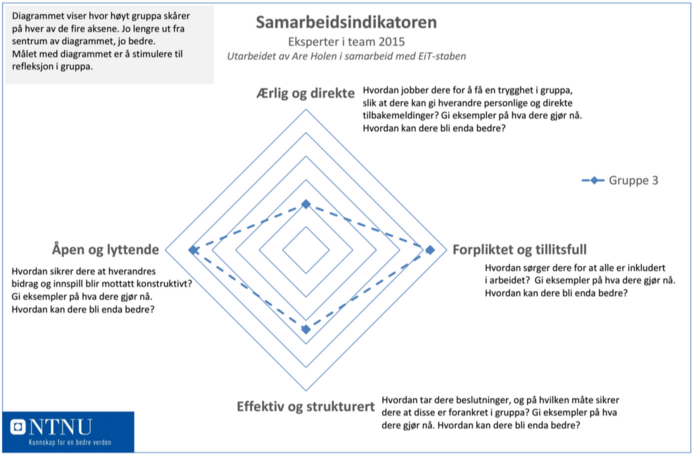
\includegraphics[width=0.5\textwidth]{Bilder/samarbeidsindikator1.png}\label{samarbeidsindikator1}

\end{figure}
\begin{figure}[h!]
  \caption{Samarbeidsindikator 2, midt i faget}
  \centering
    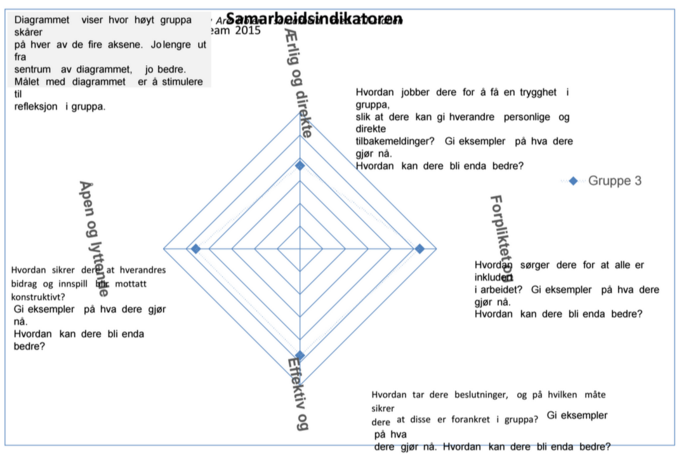
\includegraphics[width=0.5\textwidth]{Bilder/samarbeidsindikator_2.png}\label{samarbeidsindikator2}
\end{figure}

\begin{figure}[h!]
  \caption{Samarbeidsindikator 3, mot slutten av faget}
  \centering
    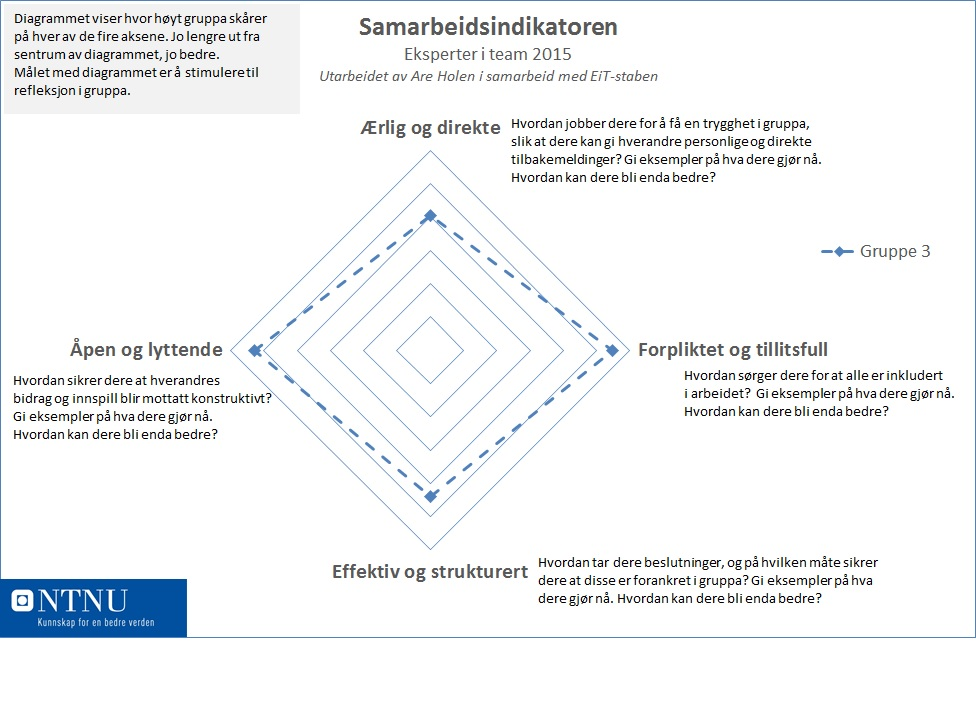
\includegraphics[width=0.5\textwidth]{Bilder/samarbeidsindikator_3.jpg}\label{samarbeidsindikator3}
\end{figure}

\emph{Åpen kommunikasjon} har gruppen hatt bra utslag på ifølge undersøkelsene siden starten av faget. 
Dette er noe gruppen har gjort bra, med unntak av oppstartsfasen (se figur \ref{samarbeidsindikator1}).
Her er det snakk om gruppens sentimenter omkring ærlig og direkte oppførsel, hvor scoren var lav.
Denne dualiteten var noe gruppen stusset over - det var overraskende at ærlighetsscoren var så lav, og dette gjorde inntrykk ved at det ble tatt opp gjentagne ganger da resultatene var klare.
Scoren for 'åpen og lyttende' atmosfære har vært vedvarende høy, og 'ærlig og direkte' gikk mot høyere score (se figurer \ref{samarbeidsindikator2}, \ref{samarbeidsindikator3}).
Gruppen reflekterte over dette, og kom frem til at det hersker en spesiell atmosfære når en gruppe er ny, og medlemmene vet at de skal samarbeide i lang tid.
Her vil det ofte være ivrighet til å skape en god stemning; folk vil le høyere av vitser som de ikke synes er så morsomme, de vil være mer tålmodige med andres bagateller, og være ekstra følsom for å levere en negativ tilbakemelding.
Gruppemedlemmene skjønner at ærlighet ofte holdes skjult under en fasade av høflighet, men skjønner også at dette gjøres for å sikre en trygg og samtalevennlig atmosfære. Det tok noen landsbydager før gruppen kunne behandle hverandes væremåte ærlig.
Et spesifikt eksempel er at Anna ventet til landsbydag fire med å kommentere at Jonas hadde en tendens til å snakke for mye, hvor det ble behandlet med rolig gemytt. 
Altså kan en gruppes sosiale samvær justeres etter hvert når medlemmene er mere komfortable med hverandre. 
Gruppen mener at den tidlige stemning var velment, men hindret ærlig og direkte kommunikasjon tidlig i prosessen, slik som samarbeidsindikatoren viser. 
Dette kunne da også ha bidratt til den trivelige sosiale atmosfæren; kanskje en startfase hvor ubehageligheter pakkes godt inn i diplomatiske utsagn er noe som skal til for å danne et trygt grunnlag.
Som samarbeidsindikatoren viser, gled gruppen inn i en meget trygg sosial atmosfære, som siden har vært en svært positiv innflytelse på gruppens samarbeid.\\
\\
\emph{Gjensidig tillit} må opparbeides. 
Det er få situasjoner hvor folk som er fremmed for hverandre og hverandres bakgrunn føler seg komfortable før interaksjon.
Tilliten i gruppen har kommet av en universell motivasjon for å jobbe sammen. 
I oppgavene i de første ukene demonstrerte gruppen viljen til å  arbeide og samarbeide.
Med en åpen og lyttende natur hvor det har vært ønsket at alle skal bli hørt, har dette ført til en atmosfære av gjensidig tillit. 
Selv når folk har kommet for sent, eller levert arbeid for sent, har det ikke vært foruroligende grunnet den underliggende tilliten.
Her kan vi også observere at en økt gjensidig tillit kan føre til at medlemmene er litt mer avslappet rundt tidsfrister.
Skulle det være fremmede eller sterkt kritiske kollegaer ville det være større grunn til sosial stress.
Dette ville da kanskje føre til at medlemmene var mere stringent med tanke på frister, men ville skape større sjanse for en potensielt destruktiv konfrontasjon.\\
\\
\emph{Sosial støtte} vokste frem stille og rolig, drevet mye av et økt sosialt velbehag, samt innsjekk og utsjekk. 
De faglig rammene for hver landsydag var grobunn for innsikt i hverandres liv. 
Derfor ble innsjekk og utsjekk alltid tatt på alvor. 
I disse 'øyeblikk' har individer fått mulighet til å vise tillit til hverandre og inkludere resten av gruppen i livet sitt. Referatene viser til en trend i å dele 'historier'; gruppen har fulgt Ingelins kvalifisering til NM i vektløftning, Simens fortellinger om sin sønn, Annas beslutning tidlig i prosessen til røykestopp og maratonløping, og Jonas sitt ansvar som hovmester på Samfundet er noen eksempler vi kan ta som viser til dette punktet.
En god sosial kommunikasjon og en trivelig tone har skapt et positivt og trygt arbeidsmiljø\cite{happy}.
Medlemmer får lyst å samarbeide og føler seg mer komfortable, hvis de føler seg verdsatt som mere enn bare et verktøy i et fag.\\
\\
\emph{Utnyttelse av individuelle forskjeller} på sosialt plan er noe annet en på et faglig plan.
Et godt sosialt miljø gjorde at medlemmene ble klar over hvilke personlighetstyper som finnes i gruppen.
Dette er informasjon som er \emph{svært viktig} i et samarbeid.
Fra begynnelsen av prosessen har hvert enkelt medlem i gruppen vært inkluderende og dedikerte til laginnsatsen. 
Dette har gjort det mye lettere å bli kjent med hverandre.
De forskjellige personlighetstypene har påvirket gruppen på hver sin måte.
I gruppen har dette vist seg ved at Jonas og Karsten har oppført seg som verv-erfarne initiativtakere,  Martin og Simen har formidlet gjennomtenkte og reflekterte utsagn, og Anna og Ingelin har hatt nøye blikk for struktur og fremdrift.
Gruppen hadde også en overordnet tendens til å fremheve den positive siden over den negative siden.
Annas usikkerheter rundt det norske språket har ikke vært til bry for gruppen, og hun føler seg tålmodig behandlet.
På samme måte \emph{kunne} det vært sett på som en negativ ting at Jonas ofte fører ordet, men gruppen la heller merke til hvor mye han bidro.
Gruppen har altså ikke latt seg irritere over ting de ikke kunne gjøre noe med, og heller vært adaptive og fokusert på fordeler og styrker.
\\